\documentclass[12pt,utf8,notheorems,compress,t]{beamer}
\usepackage{etex}

\usepackage[english]{babel}

\usepackage{mathtools}
\usepackage{booktabs}
\usepackage{stmaryrd}
\usepackage{array}
\usepackage{ragged2e}
\usepackage{multicol}
\usepackage{tabto}
\usepackage{xstring}
\usepackage{ifthen}
\usepackage{soul}\setul{0.3ex}{}
\usepackage[all]{xy}
\xyoption{rotate}
\usepackage{tikz}
\usetikzlibrary{calc,shapes,shapes.callouts,shapes.arrows,patterns,fit,backgrounds,decorations.pathmorphing}
\hypersetup{colorlinks=true}
\usepackage{multimedia}
\newcommand{\video}[2]{\movie[width=#2,height=#2,autostart,loop,poster]{}{#1}}
\hypersetup{colorlinks=false}

\usepackage{pifont}
\newcommand{\cmark}{\ding{51}}
\newcommand{\xmark}{\ding{55}}
\DeclareSymbolFont{extraup}{U}{zavm}{m}{n}
\DeclareMathSymbol{\varheart}{\mathalpha}{extraup}{86}

\graphicspath{{images/}}

\usepackage[protrusion=true,expansion=true]{microtype}

\setlength\parskip{\medskipamount}
\setlength\parindent{0pt}

\title{New reduction techniques in commutative algebra driven by logical methods}
\author{Ingo Blechschmidt}
\date{October 24th, 2018}

\useinnertheme[shadow=true]{rounded}
\setbeamerfont{block title}{size={}}

\useinnertheme{rectangles}

\usecolortheme{orchid}
\usecolortheme{seahorse}
\definecolor{mypurple}{RGB}{150,0,255}
\setbeamercolor{structure}{fg=mypurple}
\definecolor{myred}{RGB}{150,0,0}
\setbeamercolor*{title}{bg=myred,fg=white}
\setbeamercolor*{titlelike}{bg=myred,fg=white}
\setbeamercolor{frame}{bg=black}

\usefonttheme{serif}
\usepackage[T1]{fontenc}
\usepackage{libertine}

\newcommand{\A}{\mathcal{A}}
\renewcommand{\AA}{\mathbb{A}}
\newcommand{\E}{\mathcal{E}}
\newcommand{\F}{\mathcal{F}}
\renewcommand{\G}{\mathcal{G}}
\newcommand{\GG}{\mathbb{G}}
\renewcommand{\O}{\mathcal{O}}
\newcommand{\K}{\mathcal{K}}
\newcommand{\NN}{\mathbb{N}}
\newcommand{\QQ}{\mathbb{Q}}
\newcommand{\RR}{\mathbb{R}}
\newcommand{\TT}{\mathbb{T}}
\newcommand{\PP}{\mathbb{P}}
\newcommand{\ZZ}{\mathbb{Z}}
\newcommand{\CC}{\mathbb{C}}
\renewcommand{\P}{\mathcal{P}}
\newcommand{\ppp}{\mathfrak{p}}
\newcommand{\defeq}{\vcentcolon=}
\newcommand{\defeqv}{\vcentcolon\equiv}
\newcommand{\Sh}{\mathrm{Sh}}
\newcommand{\GL}{\mathrm{GL}}
\newcommand{\Zar}{\mathrm{Zar}}
\newcommand{\op}{\mathrm{op}}
\newcommand{\Set}{\mathrm{Set}}
\newcommand{\Eff}{\mathrm{Ef{}f}}
\newcommand{\Sch}{\mathrm{Sch}}
\newcommand{\Aff}{\mathrm{Aff}}
\newcommand{\LRS}{\mathrm{LRS}}
\newcommand{\Hom}{\mathrm{Hom}}
\newcommand{\Spec}{\mathrm{Spec}}
\newcommand{\lra}{\longrightarrow}
\newcommand{\RelSpec}{\operatorname{Spec}}
\renewcommand{\_}{\mathpunct{.}}
\newcommand{\?}{\,{:}\,}
\newcommand{\speak}[1]{\ulcorner\text{\textnormal{#1}}\urcorner}
\newcommand{\ull}[1]{\underline{#1}}
\newcommand{\affl}{\ensuremath{{\ull{\AA}^1}}}
\newcommand{\Ll}{\vcentcolon\!\Longleftrightarrow}
\newcommand{\inv}{inv.\@}
\newcommand{\seq}{\vdash_{\!\!\!\vec x}}

\setbeamertemplate{blocks}[rounded][shadow=false]

% Adapted from https://latex.org/forum/viewtopic.php?t=2251 (Stefan Kottwitz)
\newenvironment<>{hilblock}{
  \begin{center}
    \begin{minipage}{9.05cm}
      \setlength{\textwidth}{9.05cm}
      \begin{actionenv}#1
        \def\insertblocktitle{}
        \par
        \usebeamertemplate{block begin}}{
        \par
        \usebeamertemplate{block end}
      \end{actionenv}
    \end{minipage}
  \end{center}}

\newcommand{\bignumber}[1]{
  \renewcommand{\insertenumlabel}{#1}\scalebox{1.5}{\usebeamertemplate{enumerate item}}
}
\newcommand{\bigheart}{
\includegraphics{heart}}

\newenvironment{changemargin}[2]{%
  \begin{list}{}{%
    \setlength{\topsep}{0pt}%
    \setlength{\leftmargin}{#1}%
    \setlength{\rightmargin}{#2}%
    \setlength{\listparindent}{\parindent}%
    \setlength{\itemindent}{\parindent}%
    \setlength{\parsep}{\parskip}%
  }%
  \item[]}{\end{list}}

\tikzset{
  invisible/.style={opacity=0,text opacity=0},
  visible on/.style={alt={#1{}{invisible}}},
  alt/.code args={<#1>#2#3}{%
    \alt<#1>{\pgfkeysalso{#2}}{\pgfkeysalso{#3}}}
}

\newcommand{\pointthis}[3]{%
  \tikz[remember picture,baseline]{
    \node[anchor=base,inner sep=0,outer sep=0] (#2) {#2};
    \node[visible on=#1,overlay,rectangle callout,rounded corners,callout relative pointer={(0.3cm,0.5cm)},fill=blue!20] at ($(#2.north)+(-0.1cm,-1.1cm)$) {#3};
  }%
}

% Adapted from https://latex.org/forum/viewtopic.php?t=2251 (Stefan Kottwitz)
\newenvironment<>{varblock}[2]{\begin{varblockextra}{#1}{#2}{}}{\end{varblockextra}}
\newenvironment<>{varblockextra}[3]{
  \begin{center}
    \begin{minipage}{#1}
      \begin{actionenv}#4
        {\centering \hil{#2}\par}
	\def\insertblocktitle{}%\centering #2}
        \def\varblockextraend{#3}
	\usebeamertemplate{block begin}}{
        \par
        \usebeamertemplate{block end}
        \varblockextraend
      \end{actionenv}
    \end{minipage}
  \end{center}}

\setbeamertemplate{frametitle}{%
  \vskip1.2em%
  \leavevmode%
  \begin{beamercolorbox}[dp=1ex,center]{}%
      \usebeamercolor[fg]{item}{\textbf{{\Large \insertframetitle}}}
  \end{beamercolorbox}%
}

\setbeamertemplate{navigation symbols}{}

\newcounter{framenumberpreappendix}
\newcommand{\backupstart}{
  \setcounter{framenumberpreappendix}{\value{framenumber}}
}
\newcommand{\backupend}{
  \addtocounter{framenumberpreappendix}{-\value{framenumber}}
  \addtocounter{framenumber}{\value{framenumberpreappendix}} 
}

\newcommand{\mynav}[3]{%
  \begin{beamercolorbox}[wd=\paperwidth,ht=2.25ex]{}%
    \begin{columns}
      \begin{column}{0.333\textwidth}
        \raggedright
        \textcolor{#1}{\qquad\qquad Summary}
        \par
      \end{column}
      \begin{column}{0.333\textwidth}
        \centering
        \textcolor{#2}{The forcing model}
        \par
      \end{column}
      \begin{column}{0.333\textwidth}
        \raggedleft
        \textcolor{#3}{Revisiting the test cases \qquad\qquad}
        \par
      \end{column}
    \end{columns}
  \end{beamercolorbox}%
}

\newcommand{\insertframeextra}{}
\setbeamertemplate{footline}{%
  \begin{beamercolorbox}[wd=\paperwidth,ht=2.25ex,dp=1ex,right,rightskip=1mm,leftskip=1mm]{}%
    % \inserttitle
    \hfill
    \insertframenumber\insertframeextra\,/\,\inserttotalframenumber
  \end{beamercolorbox}%
  \vskip0pt%
}


\newcommand{\hil}[1]{{\usebeamercolor[fg]{item}{\textbf{#1}}}}
\newcommand{\bad}[1]{\textcolor{red!90}{\textnormal{#1}}}

\begin{document}

\addtocounter{framenumber}{-1}

\setbeamertemplate{headline}{\mynav{gray}{gray}{gray}}

{\usebackgroundtemplate{\begin{minipage}{\paperwidth}\vspace*{4.95cm}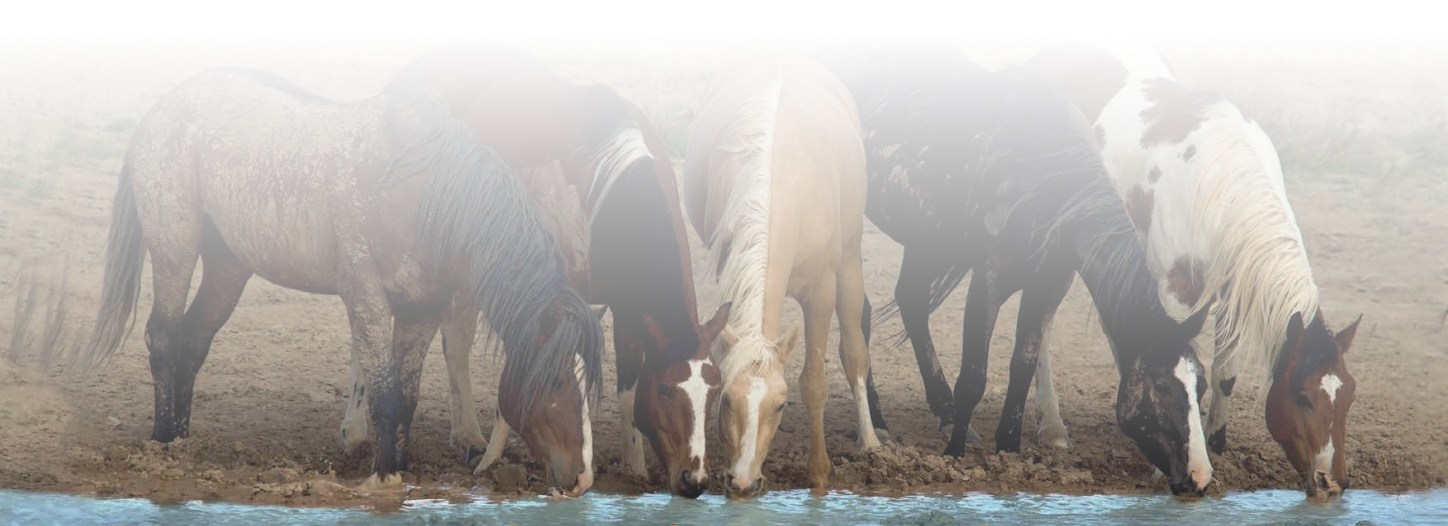
\includegraphics[width=\paperwidth]{topos-horses}\end{minipage}}
\begin{frame}[c]
  \centering

  \bigskip
  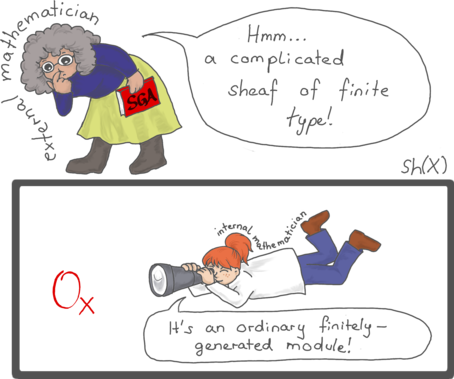
\includegraphics[width=0.4\textwidth]{external-internal-small}
  \bigskip

  \hil{New reduction techniques in commutative algebra driven by logical methods}

  \scriptsize
  \textit{-- an invitation --}
  \bigskip

  Ingo Blechschmidt \\
  Università di Verona
  \bigskip

  Logic Seminar Verona \\
  December 3rd, 2018
  \par
\end{frame}}


\section{Summary}
\setbeamertemplate{headline}{\mynav{black}{gray}{gray}}

\begin{frame}{Summary}
  \vspace*{-1em}

  \visible<4>{
    \begin{changemargin}{-2.0em}{-0.5em}
      \begin{itemize}
        \item \ \\[-1.2em]\mbox{For any reduced ring~$A$, there is a ring~$A^\sim$ in a certain topos with}
        \[ \models \bigl(\forall x\?A^\sim\_ \neg(\exists y\?A^\sim\_ xy = 1) \Rightarrow x = 0\bigr). \]

        \item This semantics is sound with respect to intuitionistic logic.

        \item \ \\[-1.2em]\mbox{It has uses in classical and constructive commutative
        algebra.}
      \end{itemize}
    \end{changemargin}
  }

  \vspace*{-1.5em}

  \begin{columns}[t]
    \begin{column}[t]{0.52\textwidth}
      \centering

      \begin{varblock}{\textwidth}{A baby example}
        \justifying
        Let~$M$ be an injective matrix with more columns than rows over a
        reduced ring~$A$.
        Then~$1 = 0$ in~$A$.
      \end{varblock}
      \vspace*{-0.5em}

      \only<1>{
        \scalebox{0.8}{$\begin{pmatrix}
          \cdot & \cdot & \cdot & \cdot & \cdot \\
          \cdot & \cdot & \cdot & \cdot & \cdot \\
          \cdot & \cdot & \cdot & \cdot & \cdot
        \end{pmatrix}$}
      }

      \visible<2->{
        \justifying
        \textbf{Proof.} \bad{Assume not.} Then there is a \bad{minimal
        prime ideal} $\ppp \subseteq A$. The matrix is injective over the \bad{field}~$A_\ppp = A[(A
        \setminus \ppp)^{-1}]$; contradiction to basic linear algebra.
      }
    \end{column}

    \begin{column}[t]{0.46\textwidth}
      \centering

      \begin{varblock}{\textwidth}{Generic freeness\phantom{p}}
        \justifying
        Generically, any finitely generated module over a reduced ring
        is free.\phantom{g}
      \end{varblock}
      \vspace*{-0.5em}

      \only<1-2>{{
        \scriptsize\raggedright
        (A ring is reduced iff $x^n=0$ implies $x=0$.)
        \par
      }}

      \only<1-2>{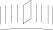
\includegraphics[width=0.73\textwidth]{generic-freeness}}

      \visible<3->{
        \justifying
        \textbf{Proof.} See [Stacks Project].
      }
    \end{column}
  \end{columns}
\end{frame}


\section{The forcing model}
\setbeamertemplate{headline}{\mynav{gray}{black}{gray}}

\begin{frame}{Motivating the semantics}
  \centering
  \begin{varblockextra}{0.8\textwidth}{}{
    \hil{Examples:}\phantom{Non-}\,\!\ \ $k,\ k[[X]],\ \CC\{z\},\ \ZZ_{(p)}$ \\[0.2em]
    \hil{Non-examples:}\ \ $\ZZ,\ k[X],\ \ZZ/(pq)$
  }
    \justifying
    A ring is \hil{local} iff~$1 \neq 0$ and if~$x + y = 1$ implies that~$x$ is
    invertible or~$y$ is invertible.
  \end{varblockextra}

  \begin{varblockextra}{0.8\textwidth}{}{
    Let~$x + y = 1$ in a ring~$A$.
    Then:
    \begin{itemize}
      \item The element $x$ is invertible in~$A[x^{-1}]$.
      \item The element $y$ is invertible in~$A[y^{-1}]$.
    \end{itemize}
  }
    \hil{Locally,} any ring is local.
  \end{varblockextra}
\end{frame}

\begin{frame}{The Kripke--Joyal semantics}
  \small
  \mbox{\!\!\!Recall~$A[f^{-1}] = \bigl\{ \frac{u}{f^n} \,|\, u \in A, n \in \NN \bigr\}$.
  Let~``$\models \varphi$'' be short for~``$1 \models \varphi$''.}
  \only<1>{\[ \renewcommand{\arraystretch}{1.25}\begin{array}{@{}l@{\quad}c@{\quad}l@{}}
    f \models \top &\text{iff}& \top \\
    f \models \bot &\text{iff}& \text{$f$ is nilpotent} \\
    f \models x = y &\text{iff}& x = y \in A[f^{-1}] \\
    f \models \varphi \wedge \psi &\text{iff}&
      \text{$f \models \varphi$ and $f \models \psi$} \\
    f \models \varphi \vee \psi &\text{iff}&
      \text{there exists a partition~$f^n = fg_1 + \cdots + fg_m$ with,} \\
    &&\quad\text{for each~$i$, $fg_i \models \varphi$ or $fg_i \models \psi$} \\
    f \models \varphi \Rightarrow \psi &\text{iff}&
      \text{for all~$g \in A$, $fg \models \varphi$ implies $fg \models \psi$} \\
    f \models \forall x\?A^\sim\_ \varphi &\text{iff}&
      \text{for all~$g \in A$ and all $x_0 \in A[(fg)^{-1}]$, $fg \models \varphi[x_0/x]$} \\
    f \models \exists x\?A^\sim\_ \varphi &\text{iff}&
      \text{there exists a partition~$f^n = fg_1 + \cdots + fg_m$ with,} \\
    &&\quad\text{for each~$i$, $fg_i \models \varphi[x_0/x]$ for some~$x_0 \in A[(fg_i)^{-1}]$}
  \end{array} \]}
  \only<2->{\[ \renewcommand{\arraystretch}{1.25}\begin{array}{@{}l@{\quad}c@{\quad}l@{}}
    f \models x = y &\text{iff}& x = y \in A[f^{-1}] \\
    f \models \varphi \wedge \psi &\text{iff}&
      \text{$f \models \varphi$ and $f \models \psi$} \\
    f \models \varphi \vee \psi &\text{iff}&
      \text{there exists a partition~$f^n = fg_1 + \cdots + fg_m$ with,} \\
    &&\quad\text{for each~$i$, $fg_i \models \varphi$ or $fg_i \models \psi$}
  \end{array} \]}

  \pause

  \begin{columns}
    \begin{column}{0.50\textwidth}
      \begin{varblock}{\textwidth}{Monotonicity}{}
        If~$f \models \varphi$, then also~$fg \models \varphi$.
      \end{varblock}
    \end{column}

    \begin{column}{0.50\textwidth}
      \begin{varblock}{\textwidth}{Locality}{}
        \justifying
        If~$f^n = fg_1 + \cdots + fg_m$ and~$fg_i \models \varphi$ for all~$i$,
        then also~$f \models \varphi$.
      \end{varblock}
    \end{column}
  \end{columns}

  \begin{columns}
    \begin{column}{0.50\textwidth}
      \begin{varblock}{\textwidth}{Soundness\phantom{p}}{}
        If~$\varphi \vdash \psi$ and~$f \models \varphi$,
        then~$f \models \psi$.
      \end{varblock}
    \end{column}

    \begin{column}{0.50\textwidth}
      \begin{varblock}{\textwidth}{Forced properties}{}
        $A \models \speak{$A^\sim$ is a local ring}$.
      \end{varblock}
    \end{column}
  \end{columns}
\end{frame}

\tikzstyle{topos} = [draw=mypurple, very thick, rectangle, rounded corners, inner sep=5pt, inner ysep=10pt]
\tikzstyle{title} = [fill=mypurple, text=white]

% Taken from Todd Lehman (CC-BY-SA) at https://tex.stackexchange.com/a/44920/32372

\newcommand{\setisprime}[1]{
  % Sets \isprime based on #1.
  \ifnum#1=1 \gdef\isprime{0} \else \gdef\isprime{1} \fi
  \foreach \sip in {2, 3,5,...,#1} {
    \pgfmathparse{\sip*\sip>#1? 1:0}
    \ifthenelse{\pgfmathresult=1}{
      % Early-out if \sip^2 > #1.
      \breakforeach
    }{
      % Otherwise test if \sip divides #1.
      \pgfmathparse{Mod(#1,\sip)==0? 1:0}
      \ifthenelse{\pgfmathresult=1}{
        \gdef\isprime{0}
        \breakforeach
      }{}
    }
  }
}

\newcommand{\setxy}[1]{
  % Sets \x and \y to loction of cell #1.
  \pgfmathtruncatemacro{\x}{Mod(#1-1,\cols)}
  \pgfmathtruncatemacro{\y}{(#1-1) / \cols}
  \pgfmathtruncatemacro{\y}{\cols - 1 - \y}
  \pgfmathparse{2.5*(\x+.5)}\let\x\pgfmathresult
  \pgfmathparse{2.5*(\y+.5)}\let\y\pgfmathresult
}

\newcommand{\numlabel}[2]{
  % Draws label #2 at cell #1.
  \setxy{\n}
  \node[fill=none, text=black] at (\x,\y) {#2};
}

\newcommand{\drawpolygon}[2]{
  % Draws polygon with #2 vertexes at cell #1.
  \setxy{#1}
  \ifthenelse{#2>1}{ % Polygon must have at least 2 sides.
    \ifthenelse{#2<30}{ % Draw polygon if it has a small number of sides.
      \filldraw (\x,\y) +(90:1)
      \foreach \drawi in {1,...,#2} {-- +(\drawi/#2*360+90:1)} -- cycle;
    }{ % Else approximate with circle.
      \filldraw (\x,\y) circle(1);
    }
  }{}
}

\newcommand{\setpolygoncolor}[1]{
  % Sets color based on #1.
  \gdef\polycolor{black}
  \ifnum#1=2\gdef\polycolor{black!50!white}\fi
  \ifnum#1=3\gdef\polycolor{yellow!95!red}\fi
  \ifnum#1=5\gdef\polycolor{yellow!0!red}\fi
  \ifnum#1=7\gdef\polycolor{blue!75!green}\fi
  \ifnum#1=11\gdef\polycolor{blue!70!red}\fi
  \ifnum#1=13\gdef\polycolor{blue!40!red}\fi
  \ifnum#1=17\gdef\polycolor{green!50!blue}\fi
  \ifnum#1=19\gdef\polycolor{green!80!black}\fi
  \ifnum#1=23\gdef\polycolor{green!50!red}\fi
  \ifnum#1=29\gdef\polycolor{yellow!50!black}\fi
  \ifnum#1=31\gdef\polycolor{orange!50!black}\fi
  \ifnum#1=37\gdef\polycolor{red!50!black}\fi
  \ifnum#1=41\gdef\polycolor{purple!50!black}\fi
  \ifnum#1=43\gdef\polycolor{blue!50!black}\fi
  \ifnum#1=47\gdef\polycolor{green!50!black}\fi
  \ifnum#1=53\gdef\polycolor{white!50!black}\fi
  \ifnum#1=59\gdef\polycolor{white!50!black}\fi
  \ifnum#1=61\gdef\polycolor{white!50!black}\fi
  \ifnum#1=67\gdef\polycolor{white!50!black}\fi
}

\newcommand{\sieve}[2]{
  \def\cols{#1}
  \def\rows{#2}
  \begin{tikzpicture}[scale=.5]
  \pgfmathtruncatemacro{\nmax}{\rows * \cols}

  \foreach \n in {1,...,\nmax} {
    \begin{scope}[fill=gray, fill opacity=.05,
                  draw=gray, draw opacity=.10,
                  line width=4]
      \drawpolygon{\n}{\n}
    \end{scope}
    \setisprime{\n}
    \ifthenelse{\isprime=1}{
      \numlabel{\n}{\bf\n}
    }{
      \def\startintensity{.33}
      \def\incrintensity{.10}
      \def\intensity{\startintensity}

      \def\m{\n}
      \pgfmathtruncatemacro{\i}{\m / 2}

      % Divide \m by \i until \m is extinguished.
      % Increment \i each time it does not divide into \m.
      \whiledo{\m>1}{
        \setisprime{\i}
        \pgfmathparse{Mod(\m,\i)==0? 1:0}
        \ifthenelse{\pgfmathresult=1\and\isprime=1}{
          \setpolygoncolor{\i}
          \begin{scope}[fill=\polycolor, fill opacity=\intensity,
                        draw=\polycolor!85!black, draw opacity=\intensity,
                        line width=\intensity*1.5]
            \drawpolygon{\n}{\i}
          \end{scope}
          \pgfmathtruncatemacro{\m}{\m / \i}
          \pgfmathparse{\intensity + \incrintensity}\let\intensity\pgfmathresult
        }{
          \pgfmathtruncatemacro{\i}{\i - 1}
          \def\intensity{\startintensity}
        }
      }
      \begin{scope}[text=black, text opacity=.5]
        \numlabel{\n}{\scriptsize\n}
      \end{scope}
    }
  }

  \end{tikzpicture}
}

%\renewcommand{\sieve}[2]{SIEVE}
%\renewcommand{\fakesieve}[2]{SIEVE}

\newcommand{\drawbox}[4]{
  \node[topos, #4] [fit = #3] (#1) {};
  \node[title] at (#1.north) {#2};
}

\newcommand{\muchstuff}{
  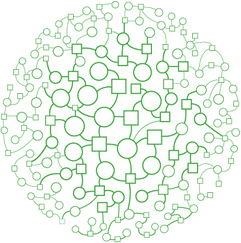
\includegraphics[height=3em]{filmat}
  \scalebox{0.5}{\sieve{14}{2}}
}

\newcommand{\muchstuffplaceholder}{
  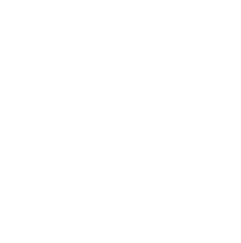
\includegraphics[height=3em]{filmat-placeholder}
  \scalebox{0.5}{\fakesieve{14}{2}}
}

\newcommand{\fewstuff}{
  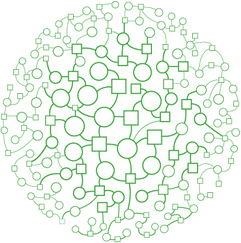
\includegraphics[height=3em]{filmat}
  \scalebox{0.5}{\sieve{7}{2}}
}

\begin{frame}[fragile]{A universal property}
  The displayed semantics is the first-order fragment of the \hil{higher-order
  internal language} of the \hil{little Zariski topos}.

  \begin{tikzpicture}
    \node[scale=0.4] (objs-set1) at (-4.0,-2.5) {
      \only<1->{\fewstuff}
    };
    \node[scale=0.4] (objs-eff1) at (4.0,-2.5) {
      \only<1->{\fewstuff}
    };
    \node[scale=0.4] (objs-sh1)  at (0,-2.5) {
      \only<1->{\fewstuff}
    };

    \node (prop-set1) [below of=objs-set1, align=left, inner ysep=0pt] {
      The usual laws \\
      of logic hold.
    };

    \node (prop-eff1) [below of=objs-eff1, align=left, inner ysep=0pt] {
      Every function \\
      is computable.
    };

    \node (prop-sh1) [below of=objs-sh1, align=left, inner sep=0pt] {
      The intermediate \\
      value theorem fails.
    };

    \begin{scope}
      \drawbox{set1}{$\mathrm{Set}$}{(objs-set1) (prop-set1)}{}
    \end{scope}
    \begin{scope}
      \drawbox{eff1}{Ef{}f}{(objs-eff1) (prop-eff1)}{tape}
    \end{scope}
    \begin{scope}
      \drawbox{sh1}{$\mathrm{Sh}\, X$}{(objs-sh1) (prop-sh1)}{draw=none}
      \def\R{8pt}
      \begin{pgfonlayer}{background}
      \draw[decoration={bumps,segment length=8pt}, decorate, very thick, draw=mypurple]
        ($(sh1.south west) + (\R, 0)$) arc(270:180:\R) --
        ($(sh1.north west) + (0, -\R)$) arc(180:90:\R) --
        ($(sh1.north east) + (-\R, 0)$) arc(90:0:\R) --
        ($(sh1.south east) + (0, \R)$) arc(0:-90:\R) --
        cycle;
      \end{pgfonlayer}
    \end{scope}
  \end{tikzpicture}

  \pause

  Is there a \hil{free local ring}~$A \to A'$ over~$A$?
  \begin{columns}[t]
    \begin{column}{0.4\textwidth}
      $\xymatrix{
        A \ar[rd] \ar[rrr]^\alpha &&& {\substack{\phantom{\text{local}}\\\text{\normalsize$R$}\\\text{local}}} \\
        & {\substack{\text{\normalsize$A'$}\\\text{local}}} \ar@{-->}_[@!35]{\text{local}}[rru]
      }$
    \end{column}

    \begin{column}{0.50\textwidth}
      \small\justifying
      For a fixed ring~$R$, the localization $A' \defeq A[S^{-1}]$ with $S \defeq
      \alpha^{-1}[R^\times]$ would do the job.
      \medskip

      Hence we need the \hil{generic filter}.
    \end{column}
  \end{columns}
\end{frame}

\begin{frame}{Investigating the forcing model}
  Let~$A$ be a reduced commutative ring ($x^n = 0 \Rightarrow x = 0$).

  The \hil{little Zariski topos} of~$A$ is equivalently
  \vspace*{-0.5em}
  \begin{itemize}
    \item the topos of sheaves over~$\Spec(A)$,
    \item the locale given by the frame of radical ideals of~$A$,
%   \item the classifying topos of local localizations of~$A$ or
    \item the classifying topos of filters of~$A$
  \end{itemize}
  \vspace*{-0.5em}
  and contains a \hil{mirror image} of~$A$, the sheaf of rings $A^\sim$.

  \vspace*{-1.5em}
  \small

  \begin{columns}
    \begin{column}{0.5\textwidth}
      \begin{varblock}{\textwidth}{}
        \justifying
        Assuming the Boolean Prime Ideal Theorem, a first-order
        formula ``$\forall \ldots \forall\_ (\cdots \Longrightarrow \cdots\!\,)$'',
        where the two subformulas may not contain~``$\Rightarrow$'' and~``$\forall$'',
        holds for~$A^\sim$ iff it holds for all stalks~$A_\ppp$.
      \end{varblock}
    \end{column}

    \begin{column}{0.5\textwidth}
      \begin{varblock}{\textwidth}{}
        $A^\sim$ inherits any property of~$A$ which is
        \hil{localization-stable}.
      \end{varblock}

      \vspace*{-1.7em}

      \setbeamercolor{block body}{bg=red!30}
      \setbeamercolor{structure}{fg=purple}
      \begin{varblock}{\textwidth}{}
        $A^\sim$ is a \hil{local ring} and a \hil{field}.

        $A^\sim$ has \hil{$\boldsymbol{\neg\neg}$-stable equality}.

        \mbox{$A^\sim$ is \hil{anonymously Noetherian}.}\\[-1.2em]
      \end{varblock}
    \end{column}
  \end{columns}

  \visible<2>{\begin{tikzpicture}[overlay]
    \draw[fill=white, draw=white, opacity=0.85] (-1,0) rectangle (\paperwidth,7.4);
    \node[anchor=south west,inner sep=0] (image) at (0,0.8) {\vbox{
      \centering
      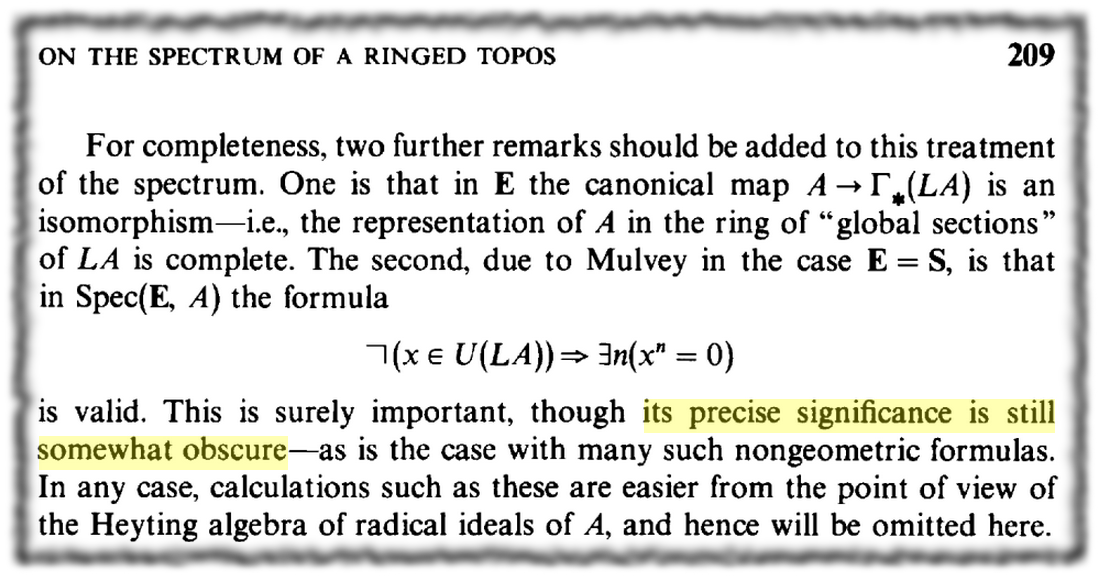
\includegraphics[width=0.9\textwidth]{tierney-on-the-spectrum-of-a-ringed-topos} \\
      \footnotesize
      Miles Tierney. On the spectrum of a ringed topos. 1976.
    }};
  \end{tikzpicture}}
\end{frame}
\renewcommand{\insertframeextra}{}


\section{Revisiting the test cases}
\setbeamertemplate{headline}{\mynav{gray}{gray}{black}}

\begin{frame}{Revisiting the test cases}
  \vspace*{-1em}
  Let~$A$ be a reduced commutative ring ($x^n = 0 \Rightarrow x = 0$). \\
  Let~$A^\sim$ be its mirror image in the little Zariski topos.

  \begin{columns}[t]
    \begin{column}[t]{0.48\textwidth}
      \centering

      \scalebox{0.5}{$\begin{pmatrix}
        \cdot & \cdot & \cdot & \cdot & \cdot \\
        \cdot & \cdot & \cdot & \cdot & \cdot \\
        \cdot & \cdot & \cdot & \cdot & \cdot
      \end{pmatrix}$}
      \vspace*{-0.5em}

      \begin{varblock}{\textwidth}{A baby example}
        \justifying
        Let~$M$ be an injective matrix over~$A$ with more columns than rows.
        Then~$1 = 0$ in~$A$.
      \end{varblock}

      \justifying
      \textbf{Proof.} $M$ is also injective as a matrix over~$A^\sim$.
      Since~$A^\sim$ is a field, this is a contradiction by basic linear
      algebra. Thus~$\models \bot$. This amounts to~$1 = 0$ in~$A$.
    \end{column}

    \begin{column}[t]{0.57\textwidth}
      \centering

      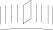
\includegraphics[height=1.9em]{generic-freeness}
      \vspace*{-0.5em}

      \begin{varblock}{\textwidth}{Generic freeness\phantom{p}}
        \justifying
        Let~$M$ be a finitely generated~$A$-module.
        If~$f = 0$ is the only element of~$A$ such that~$M[f^{-1}]$ is a
        free~$A[f^{-1}]$-module, then~$1 = 0$ in~$A$.
      \end{varblock}
      \vspace*{-0.1em}

      \justifying
      \textbf{Proof.} The claim amounts to \mbox{$\models
      \text{``$M^\sim$}$}$\text{
      is \hil{not not} free''}$. Since~$A^\sim$ is a field, this follows from
      basic linear algebra.
    \end{column}
  \end{columns}
\end{frame}


\backupstart
\setbeamertemplate{headline}{\mynav{gray}{gray}{gray}}

{\usebackgroundtemplate{\begin{minipage}{\paperwidth}\vspace*{4.95cm}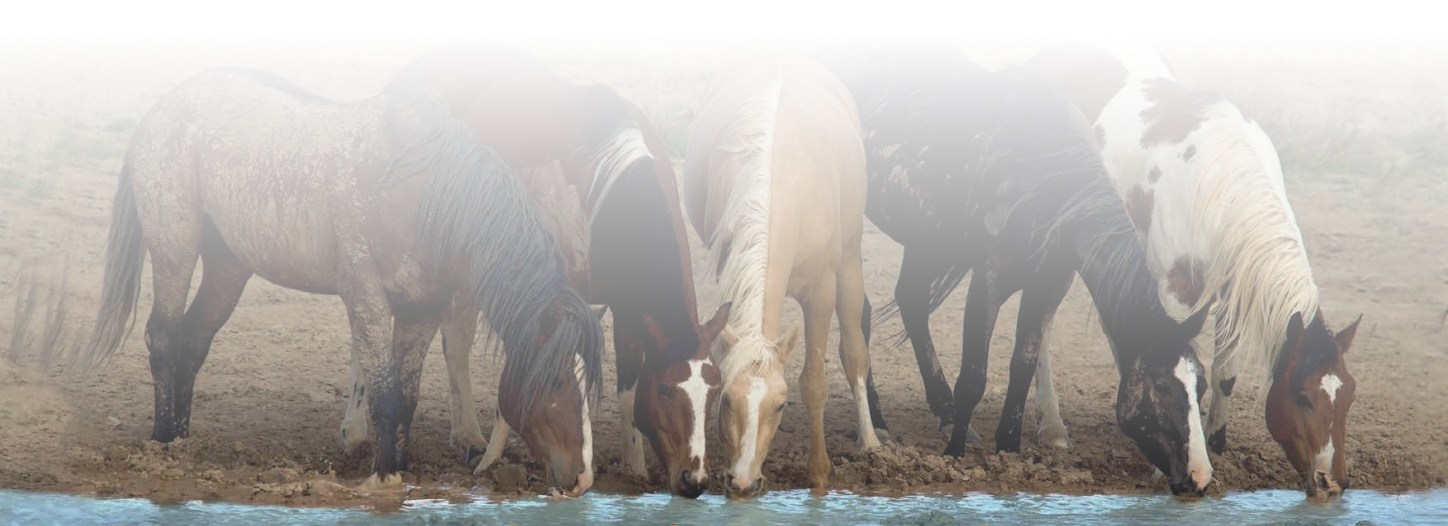
\includegraphics[width=\paperwidth]{topos-horses}\end{minipage}}
\begin{frame}
  \bigskip
  \centering
  
\includegraphics[height=3em]{heart}
  \par
  \raggedright

  The Zariski topos and related toposes have applications in:
  \begin{itemize}
    \item classical algebra and classical algebraic geometry
    \item constructive algebra and constructive algebraic geometry
    \item synthetic algebraic geometry (``schemes are just sets'')
  \end{itemize}

  Connections with:
  \begin{itemize}
    \item understanding quasicoherence
    \item the age-old mystery of nongeometric sequents
  \end{itemize}

\end{frame}}

\begin{frame}[plain,c]
  \centering%
  \hil{Further reading}
  \medskip

  \framebox{\href{https://pizzaseminar.speicherleck.de/skript2/zariski-topos-klein.pdf}{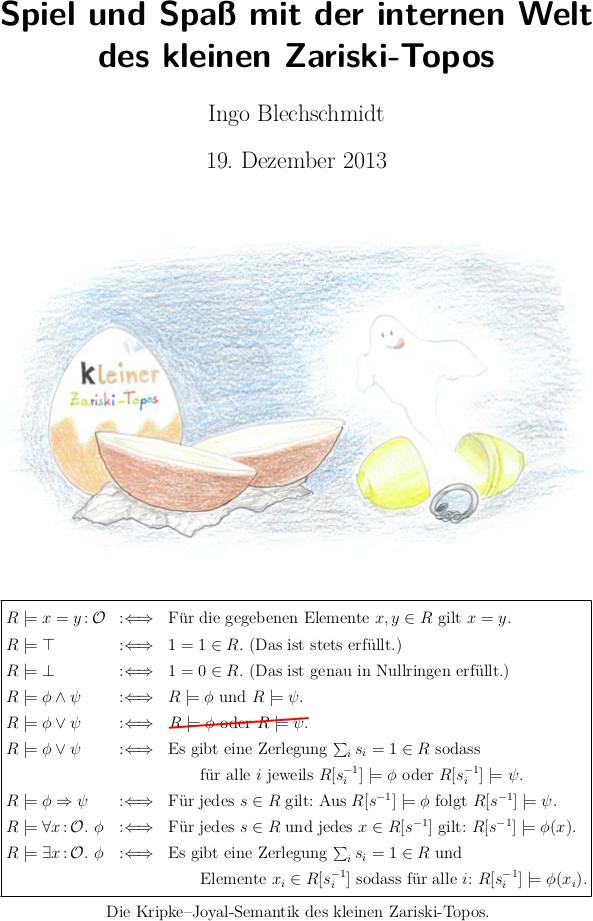
\includegraphics[height=0.8\textheight]{fun-with-the-zariski-topos}}}\qquad%
  \framebox{\href{https://rawgit.com/iblech/internal-methods/master/notes.pdf}{
\includegraphics[height=0.8\textheight]{phd-cover}}}
  \par
\end{frame}

\begin{frame}{Applications in algebraic geometry}
  \vspace*{-1.5em}
  \begin{varblock}{0.9\textwidth}{}
    \justifying
    Understand notions of algebraic geometry over a scheme~$X$ as
    notions of algebra internal to~$\Sh(X)$.
  \end{varblock}

  \small\centering
  \scalebox{0.83}{\begin{tabular}{ll}
    \toprule
    externally & internally to $\Sh(X)$ \\
    \midrule
    sheaf of sets & set \\
    %sheaf of rings & ring \\
    sheaf of modules & module \\
    sheaf of finite type & finitely generated module \\
    % finite locally free sheaf & finite free module \\
    % coherent sheaf & coherent module \\
    tensor product of sheaves & tensor product of modules \\
    % sheaf of Kähler differentials & module of Kähler differentials \\
    sheaf of rational functions & total quotient ring of~$\O_X$ \\
    dimension of $X$ & Krull dimension of~$\O_X$ \\
    spectrum of a sheaf of~$\O_X$-algebras & ordinary spectrum [with a twist] \\
    higher direct images & sheaf cohomology \\
    \bottomrule
  \end{tabular}}

  \begin{columns}[c]
    \begin{column}{0.47\textwidth}
      \begin{exampleblock}{}
        \justifying
        Let $0 \to \F' \to \F \to \F'' \to 0$ be a short exact sequence
        of sheaves of~$\O_X$-modules. If~$\F'$ and~$\F''$ are of finite type,
        so is~$\F$.
      \end{exampleblock}
    \end{column}

    \begin{column}{0.1\textwidth}
      \vspace*{0.7em}
      \scalebox{3}{$\Leftarrow$}
    \end{column}

    \begin{column}{0.44\textwidth}
      \begin{exampleblock}{}
        \justifying
        Let~$0 \to M' \to M \to M'' \to 0$ be a short exact sequence of
        modules. If~$M'$ and~$M''$ are finitely generated, so is~$M$.
      \end{exampleblock}
    \end{column}
  \end{columns}
\end{frame}

\begin{frame}{Synthetic algebraic geometry}
  Usual approach to algebraic geometry: \hil{layer schemes above ordinary set theory}
  using either
  \begin{itemize}
    \item locally ringed spaces
    \small
    \begin{multline*}
      \text{set of prime ideals of~$\ZZ[X,Y,Z]/(X^n+Y^n-Z^n)$} + {} \\
      \text{Zariski topology} + \text{structure sheaf}
    \end{multline*}
    \normalsize
    \item or Grothendieck's functor-of-points account, where a scheme is a functor~$\mathrm{Ring} \to \mathrm{Set}$.
    \small\[ A \longmapsto \{ (x,y,z) \in A^3 \,|\, x^n+y^n-z^n=0 \} \]
  \end{itemize}
  \bigskip

  \hil{Synthetic approach:} model schemes \hil{directly as sets} in a certain
  nonclassical set theory, the internal universe of the \mbox{\hil{big Zariski
  topos}} of a base scheme.
  \small
  \[ \{ (x,y,z) \? (\affl)^3 \,|\, x^n+y^n-z^n=0 \} \]
\end{frame}

\backupend

\end{document}
